\begin{center}
    \section*{\fontsize{20}{20}\selectfont Chapter 3}
\end{center}
\vspace{10mm}
\section{Research Methodology}

This chapter outlines the research methodology and the systematic approach used to develop the automated potato leaf disease detection system. It covers the feasibility analysis, the requirement specifications and the workflow from data collection to the final advisory output. The core of the chapter describes the proposed Custom Lightweight CNN and the ResNet50 and MobileNetV2 models used for comparison. Finally, the integration of Explainable AI (XAI) and the LLM-based advisory module is discussed.

\subsection{Feasibility Analysis}
Before initiating the development, a thorough feasibility study was conducted to determine the viability of the project.

\subsubsection{Technical Feasibility}
The project is technically feasible because it uses open-source and well-documented technologies. Python is the main programming language, with TensorFlow 2.20 and Keras as the deep learning frameworks \cite{abadi2016tensorflow}. The experiments were run in a Kaggle cloud notebook. The platform supports GPU acceleration, but in the reported run CUDA could not be initialized, so training ran on the CPU. This was enough to complete the full pipeline, but it limited the number of training epochs.

\subsubsection{Operational Feasibility}
The proposed system is designed to be fully automated. Once trained, the model needs minimal human intervention: users upload an image, and the system outputs the disease class, the confidence score and LLM-generated advice. This simplicity makes the system accessible to non-technical users such as farmers or agricultural extension workers.

\subsubsection{Economic Feasibility}
The project is economically viable because it relies on open-source tools (Python, TensorFlow, Jupyter and Kaggle Notebooks) that need no licensing fees. The proposed lightweight model is small enough to run on standard consumer hardware, and the LLM is called only once per prediction, so the running cost of the advisory module stays low.

\subsection{Requirement Analysis}
To ensure the successful development of the system, specific functional and non-functional requirements were defined.

\subsubsection{Functional Requirements}
\begin{itemize}
    \item \textbf{Input:} The system must accept leaf images in standard formats (JPG, PNG).
    \item \textbf{Processing:} The system must preprocess the image (resize, normalize) and pass it through the trained Deep Learning models.
    \item \textbf{Output:} The system must predict one of the 7 classes and display the confidence percentage.
    \item \textbf{Visualization:} The system must generate a Grad-CAM heatmap to visualize the infected regions used for prediction \cite{selvaraju2017grad}.
    \item \textbf{Advisory:} The system must generate farmer-friendly advice for the predicted class through the LLM, with a warning when the confidence is low.
\end{itemize}

\subsubsection{Non-Functional Requirements}
\begin{itemize}
    \item \textbf{Accuracy:} The model should achieve a testing accuracy of greater than 95\%.
    \item \textbf{Latency:} The inference time (prediction speed) should be minimal, ideally under 100 ms per image for real-time applicability.
    \item \textbf{Scalability:} The architecture should be adaptable to include new disease classes in the future.
\end{itemize}

\subsubsection{Dataset Requirements}
The research uses the Potato Leaf Disease Dataset in Uncontrolled Environment, available on Kaggle \cite{shabrina2024novel}:
\begin{itemize}
    \item \textbf{Total Images:} 3,076 images.
    \item \textbf{Classes:} 7 classes (Bacteria, Fungi, Healthy, Nematode, Pest, Phytopthora and Virus).
    \item \textbf{Format:} RGB field photographs of varying resolutions with complex backgrounds.
\end{itemize}

\subsubsection{Hardware Requirements}
\textbf{Development/Training Phase:}
\begin{itemize}
    \item \textbf{CPU:} Intel Core i5 or higher / Ryzen 5 / Cloud vCPU.
    \item \textbf{RAM:} 16 GB or higher.
    \item \textbf{GPU:} NVIDIA GPU with at least 12 GB VRAM (required for faster training).
\end{itemize}

\noindent \textbf{Deployment/Inference Phase:}
\begin{itemize}
    \item \textbf{Processor:} Standard Mobile CPU (Snapdragon/MediaTek) or Laptop CPU.
    \item \textbf{RAM:} 4 GB sufficient for the lightweight model.
\end{itemize}

\subsection{Research Model \& Methodology}
The overall workflow of the proposed methodology is illustrated in Figure~\ref{fig:workflow}.

\begin{figure}[htbp]
\centering
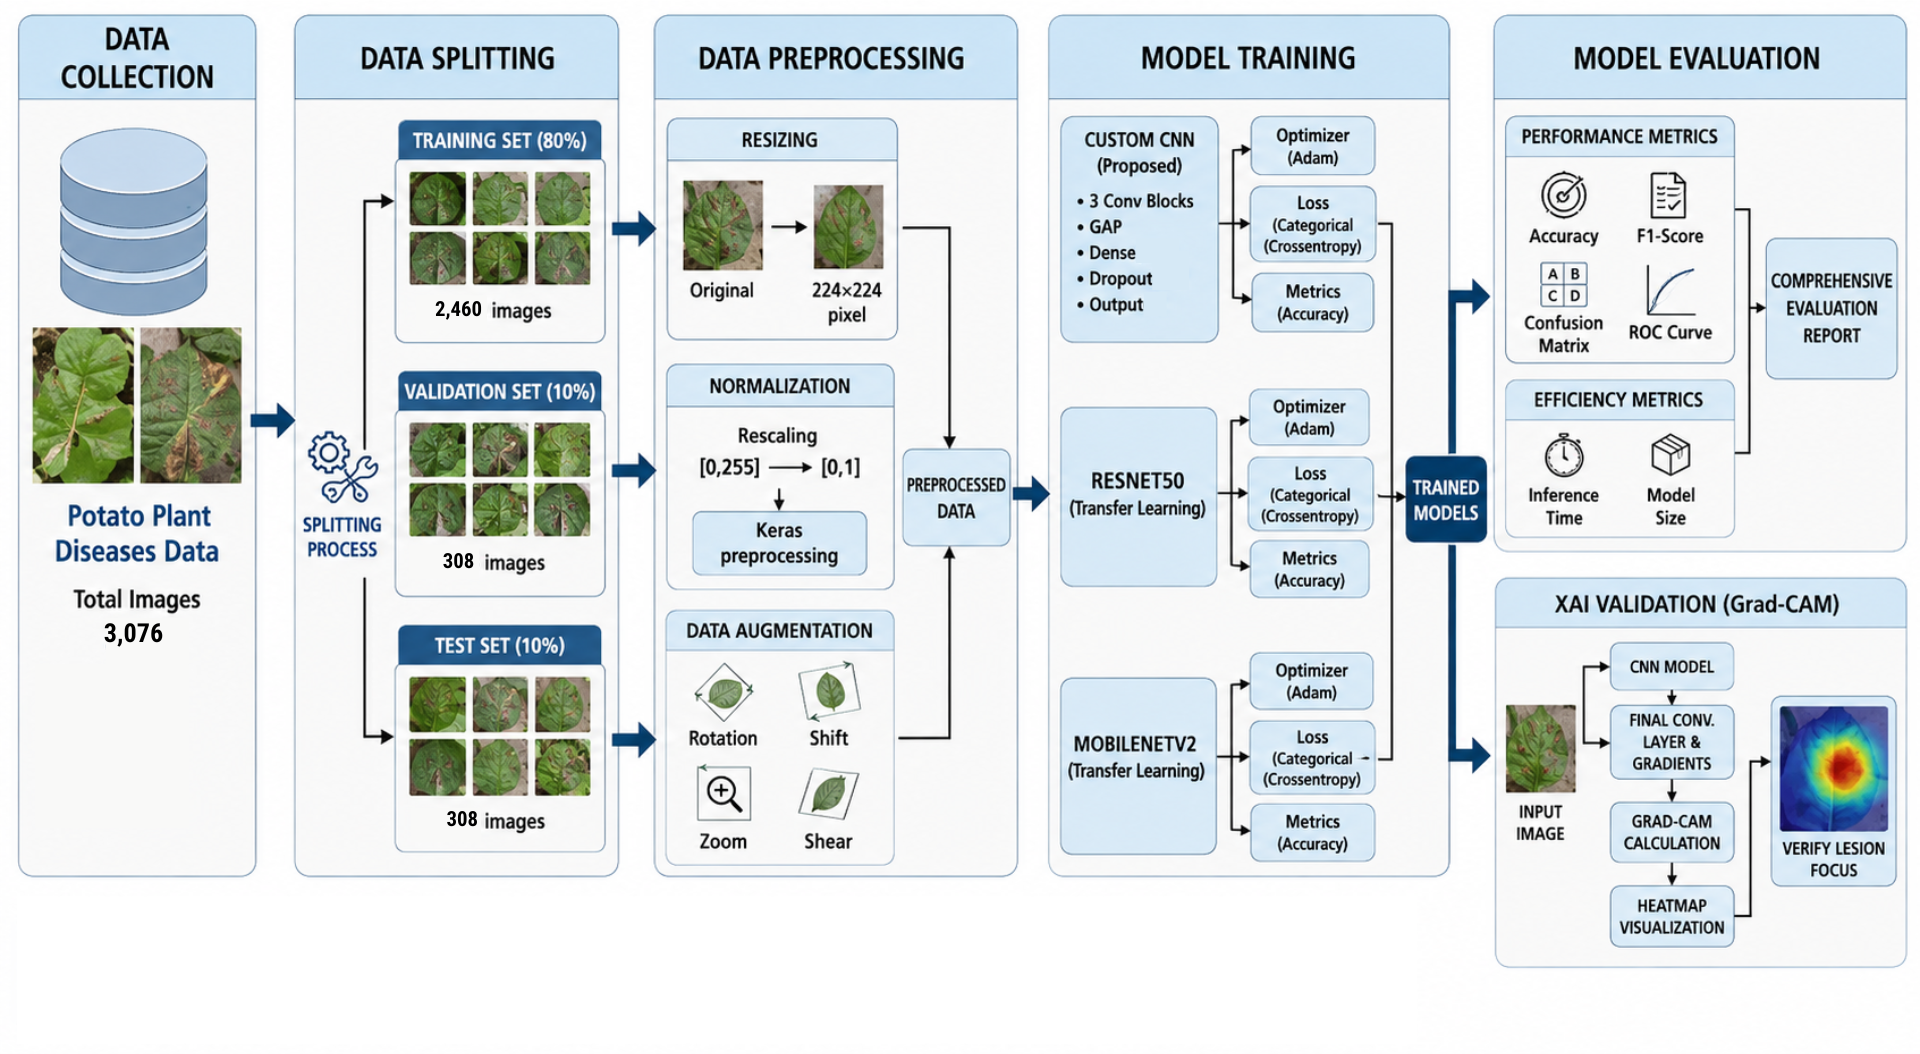
\includegraphics[width=0.95\textwidth]{image/docx_image2.png}
\caption{Workflow Diagram (Block Diagram of Proposed Methodology).}
\label{fig:workflow}
\end{figure}

\subsubsection{Data Collection}
The dataset was obtained from Kaggle (Potato Leaf Disease Dataset in Uncontrolled Environment) \cite{shabrina2024novel}. It contains 3,076 potato leaf images taken in real fields, with soil, plastic mulch, hands and other plants in the background. The images belong to 7 classes, and the class sizes are not balanced: Fungi has 748 images, while Nematode has only 68. The file paths and labels were collected into a Pandas DataFrame for processing.

\subsubsection{Data Preprocessing}
Data preprocessing is critical for model performance. The following steps were applied:
\begin{itemize}
    \item \textbf{Resizing:} All images were resized to a fixed dimension of $224 \times 224$ pixels to match the input layer of the CNN architectures.
    \item \textbf{Normalization:}
    \begin{itemize}
        \item For the Custom CNN, pixel values were rescaled from $[0, 255]$ to $[0, 1]$ by dividing by $255.0$.
        \item For ResNet50 and MobileNetV2, the model-specific Keras \texttt{preprocess\_input} functions were used (mean subtraction for ResNet50 and scaling to $[-1, 1]$ for MobileNetV2).
    \end{itemize}
    \item \textbf{Data Augmentation:} To prevent overfitting and improve generalization, we applied on-the-fly augmentation using \texttt{ImageDataGenerator} \cite{shorten2019survey}. Techniques included: rotation range of 20 degrees, width/height shift of 20\%, horizontal flip, and zoom range of 20\% (new pixels filled with the nearest value).
\end{itemize}

\subsubsection{CNN Architecture (Proposed Custom Model)}
We proposed a Custom Lightweight CNN Model designed specifically for this task. The architecture aims to reduce the number of parameters while maintaining high feature extraction capability:
\begin{itemize}
    \item \textbf{Input Layer:} Accepts images of shape $(224, 224, 3)$.
    \item \textbf{Convolutional Blocks:} The model consists of 3 main blocks. Each block contains:
    \begin{itemize}
        \item Two \texttt{Conv2D} layers with $3 \times 3$ filters (16 and 32, 32 and 64, and 64 and 128 filters).
        \item \texttt{BatchNormalization} for training stability \cite{ioffe2015batch}.
        \item Swish activation function (chosen over ReLU for better gradient flow) \cite{ramachandran2017swish}.
        \item \texttt{MaxPooling2D} for dimensionality reduction.
        \item Dropout (0.20, 0.20 and 0.25) to prevent overfitting \cite{srivastava2014dropout}.
    \end{itemize}
    \item \textbf{Global Average Pooling (GAP):} Instead of flattening the feature map, which causes a parameter explosion, GAP is used. It is followed by a Dense layer of 128 neurons with Batch Normalization, Swish and Dropout (0.40).
    \item \textbf{Output Layer:} A Dense layer with 7 neurons and Softmax activation for multi-class classification.
\end{itemize}

\subsubsection{ResNet50 Architecture}
For comparative analysis, we employed ResNet50, a deep Residual Network \cite{he2016deep}:
\begin{itemize}
    \item \textbf{Mechanism:} It uses ``skip connections'' to allow gradients to flow through the network easily, enabling the training of very deep networks (50 layers).
    \item \textbf{Configuration:} The top layers were removed, and a custom classification head (Global Average Pooling, Dense(64), Batch Normalization, Swish, Dropout(0.3) and Dense(7)) was added. The base was frozen. Because the Kaggle session could not download ImageNet weights, the base was created with random weights (\texttt{weights = None}), so this run is not true transfer learning.
\end{itemize}

\subsubsection{MobileNetV2 Architecture}
We also implemented MobileNetV2, a model optimized for mobile devices \cite{howard2017mobilenets}:
\begin{itemize}
    \item \textbf{Mechanism:} It uses Depthwise Separable Convolutions and Inverted Residual Blocks. This significantly reduces the number of operations (FLOPs) and parameters compared to standard CNNs.
    \item \textbf{Configuration:} The same classification head as ResNet50 was attached. Since no pre-trained weights were loaded (\texttt{weights = None}), all MobileNetV2 layers were set as trainable, so that the network could learn features from the potato images.
\end{itemize}

\subsubsection{Model Evaluation}
The models were evaluated using a comprehensive set of metrics \cite{grandini2020metrics}:
\begin{itemize}
    \item \textbf{Accuracy:} The percentage of correctly classified images.
    \item \textbf{Loss:} Categorical Crossentropy loss with label smoothing (0.1) to measure prediction error.
    \item \textbf{Precision, Recall, and F1-Score:} To evaluate performance on individual classes.
    \item \textbf{Confusion Matrix:} To visualize misclassifications between similar diseases.
    \item \textbf{ROC Curve:} To analyze the trade-off between True Positive Rate and False Positive Rate.
    \item \textbf{Efficiency Metrics:} Inference time (ms/image) and Model Size (MB).
\end{itemize}

\subsubsection{XAI with CNN (Grad-CAM)}
To address the ``black-box'' nature of CNNs, we implemented Gradient-weighted Class Activation Mapping (Grad-CAM) \cite{selvaraju2017grad}:
\begin{itemize}
    \item \textbf{Principle:} Grad-CAM uses the gradients of the target class flowing into the final convolutional layer to produce a coarse localization map highlighting the important regions in the image.
    \item \textbf{Implementation:} The feature maps of the last \texttt{Conv2D} layer are weighted by the averaged gradients of the predicted class. The resulting heatmap is resized and superimposed on the original image to check whether the model focuses on the disease lesions or on the background.
\end{itemize}

\subsubsection{LLM-Based Advisory Integration}
To make the prediction useful for farmers, the CNN output is passed to a Large Language Model (Google Gemini, model \texttt{gemini-3.1-flash-lite}) through the \texttt{google-genai} Python library \cite{google2026gemini}:
\begin{itemize}
    \item \textbf{Input:} The predicted class name and the confidence score from the CNN.
    \item \textbf{Prompt:} The LLM is asked to explain the disease name, what the disease is, common symptoms, possible causes, management steps, prevention methods and an important caution.
    \item \textbf{Safety Rules:} The LLM must not invent pesticide doses, must tell the farmer to follow the product label and local experts, must not claim that the prediction is 100\% certain, and must ask for verification when the confidence is low.
    \item \textbf{Security:} The API key is read from Kaggle Secrets and is not written in the code.
\end{itemize}

\subsection*{Summary}
This chapter presented the research methodology, including feasibility and requirement analyses, dataset preparation, the architectures of the Custom Lightweight CNN, ResNet50, and MobileNetV2, as well as the Grad-CAM explainability and Gemini LLM advisory pipelines. The next chapter details the implementation and experimental results.

\clearpage
